\documentclass{ecam}

\usepackage[utf8]{inputenc}
\usepackage[french]{babel}
\usepackage[T1]{fontenc}
\usepackage{lmodern}
\usepackage{graphicx}

% Change font to sans-serif
\renewcommand\familydefault{\sfdefault}

% Chapter title customization
\usepackage{titlesec, blindtext, color}
\definecolor{gray75}{gray}{0.75}
\newcommand{\hsp}{\hspace{20pt}}
\titleformat{\chapter}[hang]{\Huge\bfseries}{\thechapter\hsp\textcolor{gray75}{|}\hsp}{0pt}{\Huge\bfseries}
\titlespacing*{\chapter}{0pt}{30pt}{15pt}

\usepackage{etoolbox}
\makeatletter
\patchcmd{\chapter}{\if@openright\cleardoublepage\else\clearpage\fi}{}{}{}
\makeatother

% table padding
\renewcommand{\arraystretch}{1.5}

% Appendix chapters
\usepackage{appendix}

% Paragraph spacing
\setlength{\parindent}{0em}
\setlength{\parskip}{1em}

% Lists
\usepackage[shortlabels]{enumitem}

% Allows rendering images 'here' with the H option
\usepackage{float}

% Code syntax highlighting
\usepackage{minted}



\begin{document}
% Title
\title{Projet Génie logiciel \\\vspace{10pt}\fontsize{30pt}{60pt}\selectfont{KitBox}}
\author{William De Decker \& Mathieu David \& Saïkou Barry Ahmadou \linebreak \& Jonathan Petit \& Momo Guy Donatien}
\maketitle

\chapter{Diagrammes}
Les diagrammes \textit{UML} suivants sont les représentations de notre application
\textbf{KitBox} faisant l'objet du projet Génie Logiciel.

Le premier diagramme est celui des cas d'utilisation, montrant
les actions que les différents intervenants pourront réaliser au travers
de notre application.

Le diagramme de classes est la représentation des interactions entre les
différentes parties du code. Ce diagramme permet d'avoir une vision globale
des relations entre les classes et des types d'objets.

Le diagramme de séquence permet de se représenter le déroulement de l'action de
composition d'une armoire sous forme de messages entre les différentes entités
mises en jeu (système, base de données et le client). Celui-ci apporte un schéma
des différentes méthodes qui devront être présent dans l'application. Il est
complémentaire à notre diagramme de classes.

Le diagramme d'activité métier est la représentation du déroulement général d'une
commande d'armoire par le client. Il permet d'avoir une vision plus présice des
actions effectuées par les différents acteurs lors de la commande d'une armoire.

Enfin, le diagramme d'entité-relation quant à lui représente les tables dans la base
donnée et les relations qu'elles ont entre elles.

\section{Diagramme des cas d'utilisation}
\begin{center}
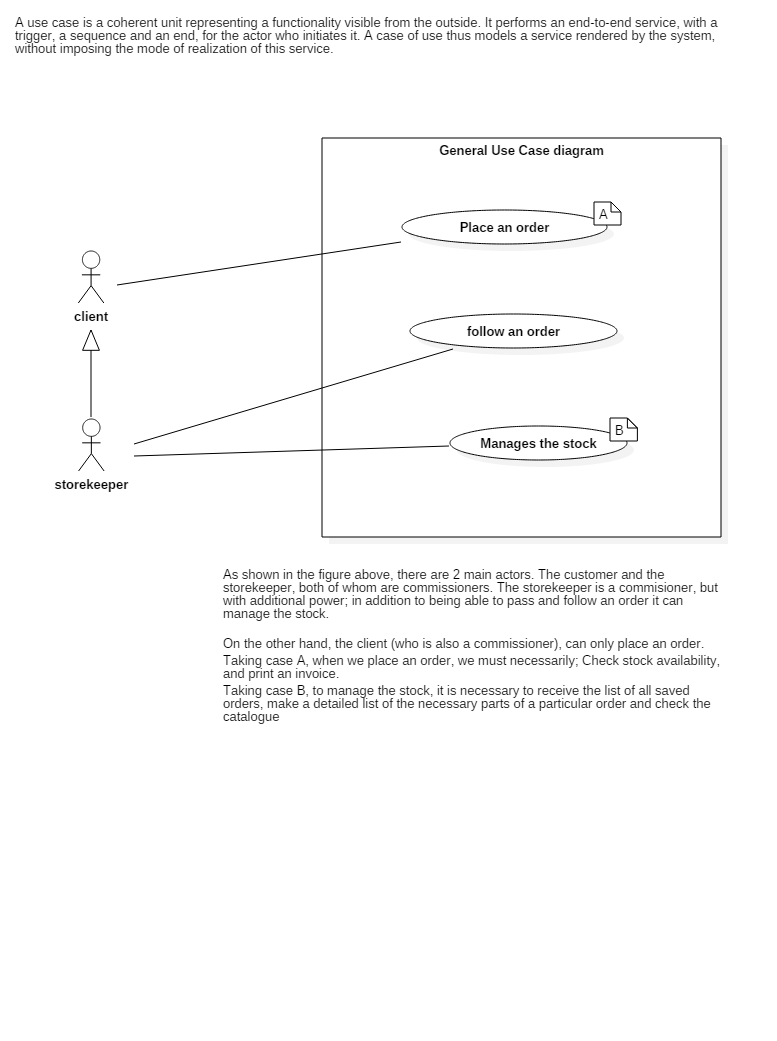
\includegraphics[angle=0,scale=0.5]{../images/use-case-diagram.png}
\end{center}

\section{Diagramme de classe}
\begin{center}
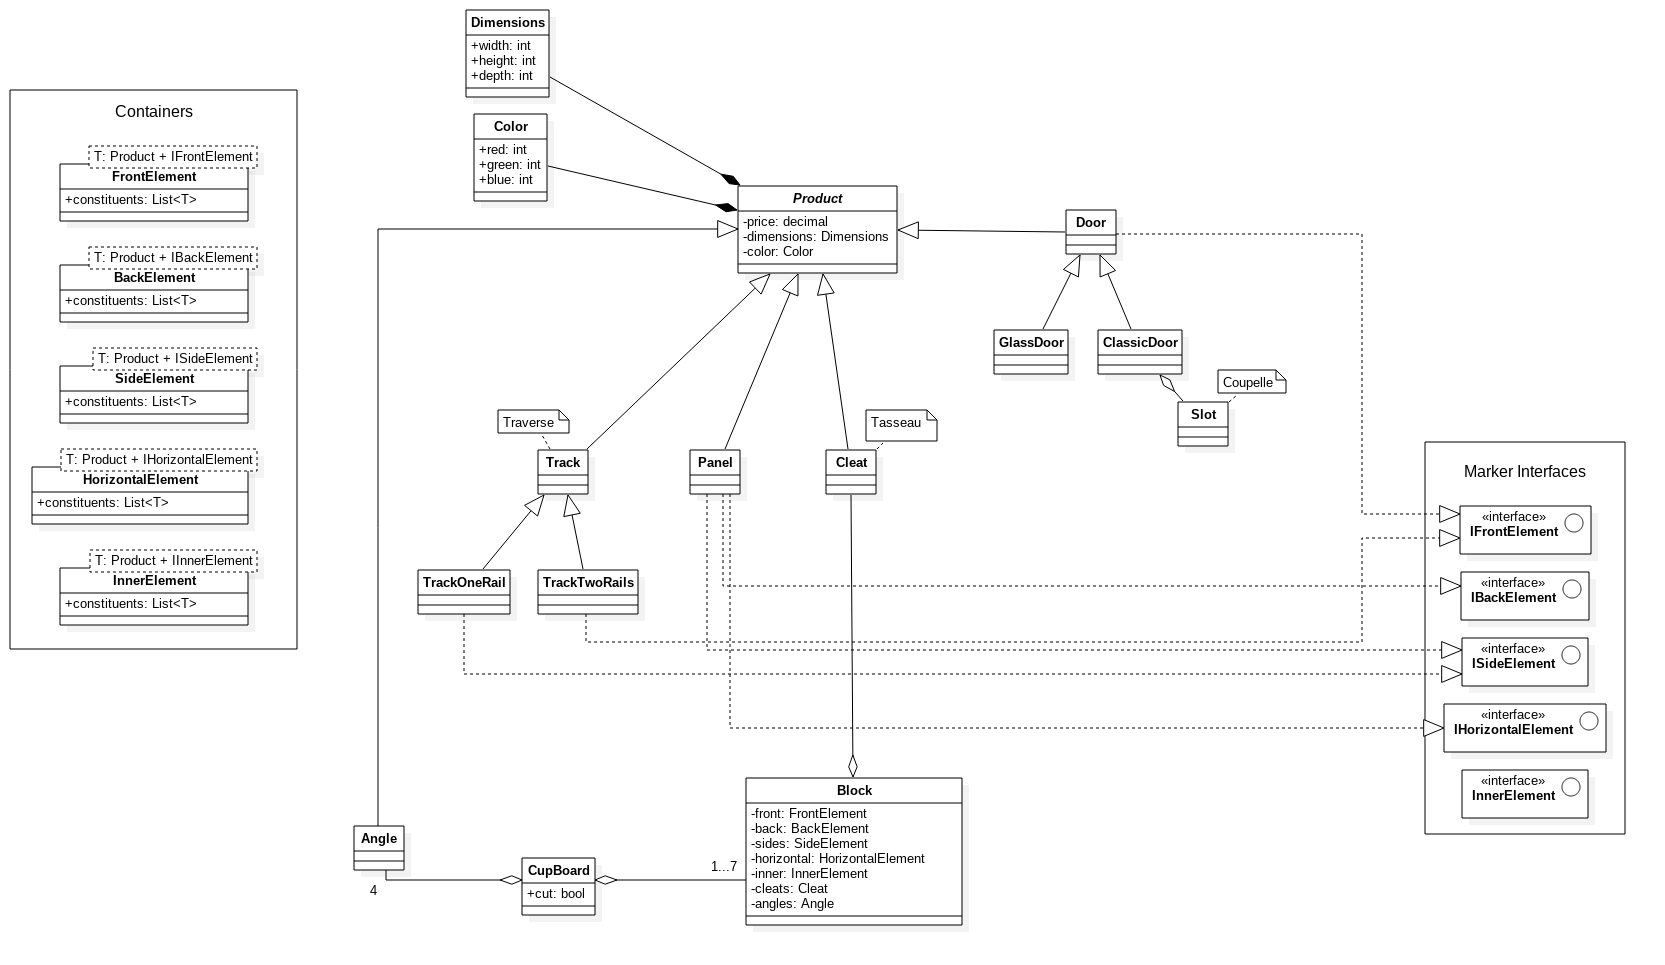
\includegraphics[angle=270,scale=0.35]{../images/class-diagram.png}
\end{center}

\section{Diagramme de Séquence}
\begin{center}
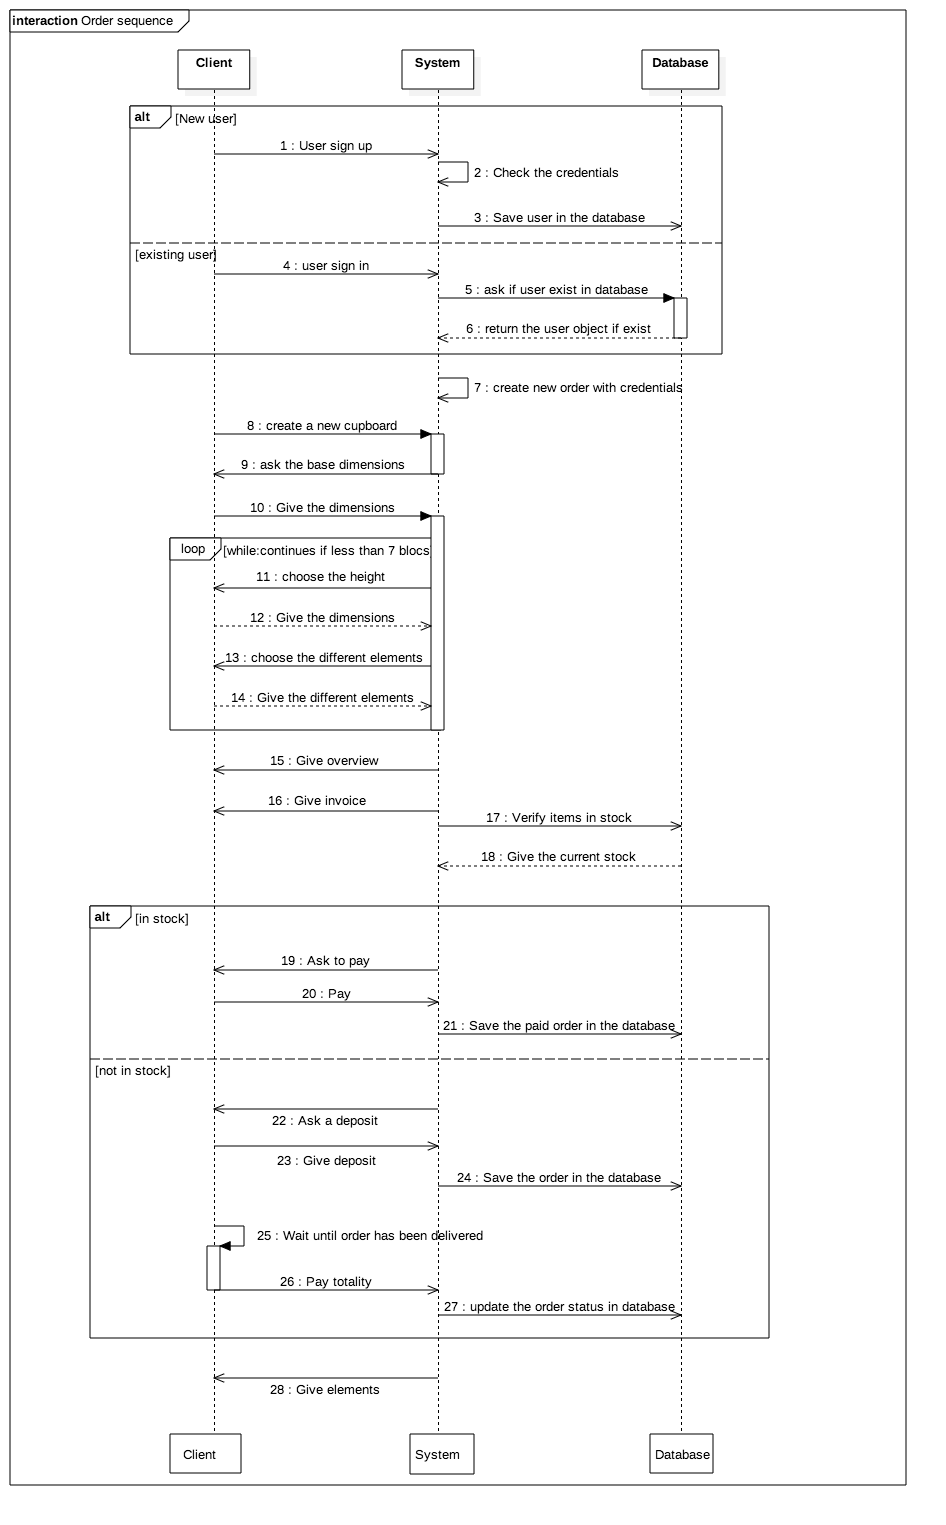
\includegraphics[scale=0.4]{../images/sequence-diagram.png}
\end{center}

\section{Diagramme d'activité}
\begin{center}
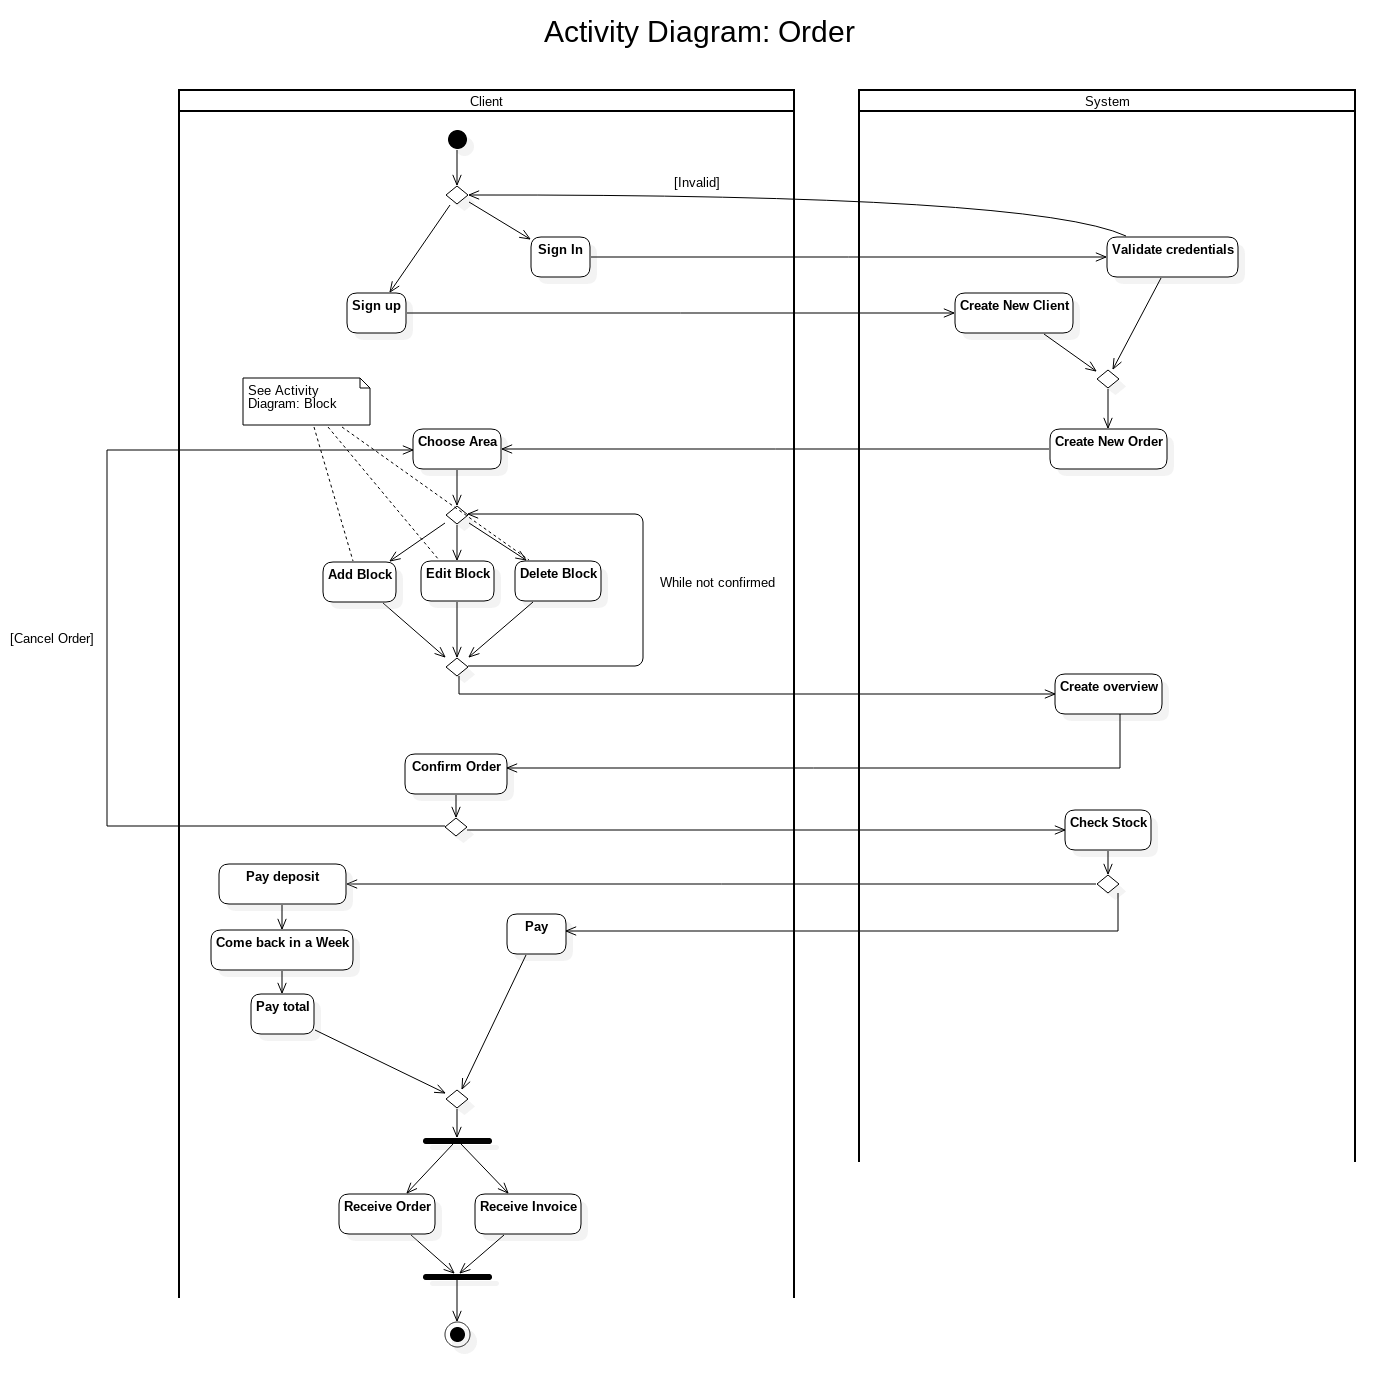
\includegraphics[angle=0,scale=0.3]{../images/activity-diagram.png}
\end{center}

\section{Diagramme d'entité-relation}
\begin{center}
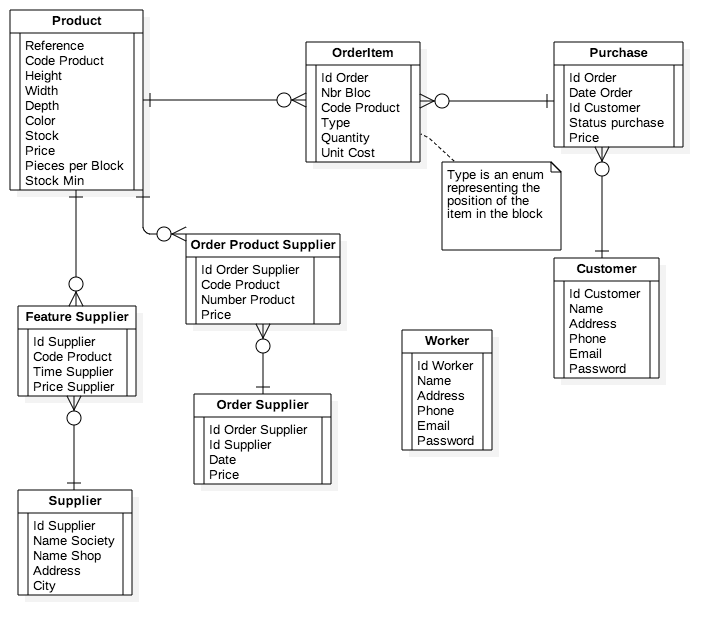
\includegraphics[angle=0,scale=0.4]{../images/ERDDiagram.png}
\end{center}

\end{document}
